\documentclass{article} 
% \usepackage[utf8]{inputenc}
\usepackage{ amssymb, systeme, mathtools,   graphicx, titlesec}
\usepackage[framemethod=tikz]{mdframed}
\usepackage{fontawesome5}

\usepackage[legalpaper,margin=1in]{geometry}

\setlength{\parindent}{10pt}
\setlength{\parskip}{1em}
\renewcommand{\baselinestretch}{1.2}

\title{PARTIAL DERIVATIVES}
\date{}
\author{}

\DeclarePairedDelimiter\abs{\lvert}{\rvert}
\DeclarePairedDelimiter\norm{\lVert}{\rVert}
\makeatletter 
\let\oldabs\abs
\def\abs{\@ifstar{\oldabs}{\oldabs*}}

\let\oldnorm\norm
\def\norm{\@ifstar{\oldnorm}{\oldnorm*}}
\makeatother
\usepackage{tabularray}


\newcounter{Def}[section]
\newenvironment{Def}[1][]{%
  \ifstrempty{#1}%
  {\mdfsetup{%
    frametitle={%
      \tikz[baseline= (current bounding box.east),outer sep=0pt]
      \node[line width=1pt,anchor=east,rectangle,draw=blue!20,fill=white]
      {\strut \color{black}{Definition}~};}}
  }%
  {\mdfsetup{%
    frametitle={%
      \tikz[baseline= (current bounding box.east),outer sep=0pt]
      \node[line width=1pt,anchor=east,rectangle,draw=blue!20,fill=white]
    {\strut \color{black}{Definition}~:~\color{blue4}{#1}};}}%
  }%
  \mdfsetup{innertopmargin=2pt,linecolor=blue!20,%
            linewidth=1pt,topline=true,%
            frametitleaboveskip=\dimexpr-\ht\strutbox\relax,}
  \begin{mdframed}[]\relax%
  }{\end{mdframed}}
%{\fontfamily{cmtt}\selectfont }
\titleformat{\section}
  {\fontfamily{lmss}\selectfont\LARGE\bfseries\color{black}}
  {\thesection}{1em}{}
\begin{document}
\section{Partial Derivatives}
Suppose we let $x$ vary while keeping $y$ fixed ($y = b$) in $f(x,y)$, we got a function $g(x) = f(x,b)$. If $g$ has a derivative at $a$, we call it the \textbf{partial derivative of \textit{f} with respect to \textit{x} at \textit{(a,b)}}. We have 
\[g'(a) = \lim_{h \to  0 }\frac{g(a + h) - g(a)}{h }\]
and so it become $\quad$
\begin{minipage}[]{0.6\linewidth}
\begin{mdframed}
\[f_x (x,y) = \lim_{h \to 0} \frac{f(x + h, b) - f(x,y)}{h }\]
\[f_y (x,y) = \lim_{h \to 0} \frac{f(x , y + h) - f(x,y)}{h }\]
  \end{mdframed}
\end{minipage}

To compute partial derivatives, we have the following rule.
\begin{mdframed}
  {\fontfamily{lmtt}\selectfont \textbf{\textcolor{blue5}{\small $\blacksquare$ Rule for Finding Partial Derivatives of $z = f(x,y)$}}} \\
{\fontfamily{lmtt}\selectfont \textbf{\small 1.}} To find $f_x$, regard $y$ as a constant and differentiate $f(x,y)$ with respect to $x$.\\
{\fontfamily{lmtt}\selectfont \textbf{\small 2.}} To find $f_y$, regard $x$ as a constant and differentiate $f(x,y)$ with respect to $y$.
\end{mdframed}
{\fontfamily{lmtt}\selectfont \textbf{\textcolor{blue5}{{\small \faIcon{map-marker-alt}} EXAMPLE.}}} If $f(x,y) = x^3 + x^2 y^3 - 2y^2$, find $f_x(2,1)$ and $f_y(2,1)$.
Holding $y$ constant and differentiating with respect to $x$, we get 
\begin{equation*}
  \begin{split}
 &   f_x(x,y) = 3 x^2 + 2x y^3 \\
 &  f_x(2,1) = 3 \cdot 2^2 + 2 \cdot 2 \cdot 1^3 = 16
  \end{split}
\end{equation*}
Do the same with $y$
\begin{equation*}
  \begin{split}
    & f_y (x,y) = 3 x^2 y^2 - 4y \\
    & f_y (2,1) = 3 \cdot 2^2 \cdot 1^2 - 4 \cdot 1 = 8       
  \end{split}
\end{equation*}

\subsection*{{\fontfamily{lmss}\selectfont \underline{Interpretations of Partial Derivatives}}}

\begin{minipage}[]{0.34\linewidth}
  \begin{center}
    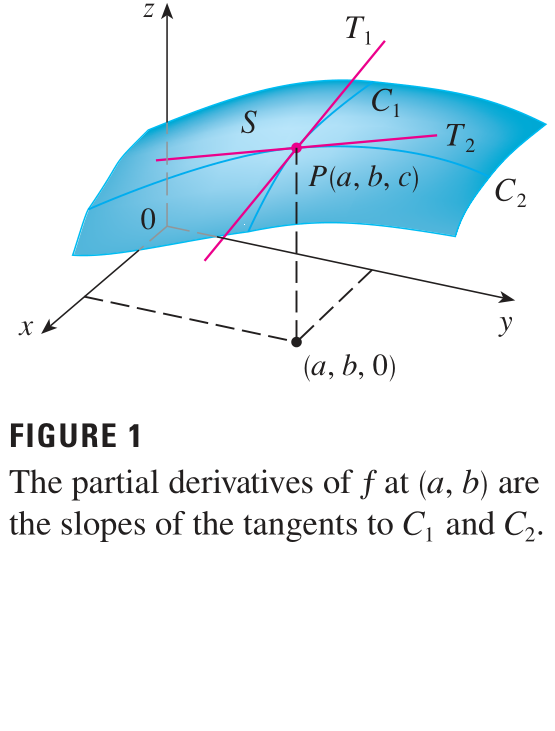
\includegraphics[width = 4.3 cm]{./images/interpretation.png} 
  \end{center}
\end{minipage}
\begin{minipage}[]{0.6\linewidth}
\textcolor{blue5}{\small $\blacksquare$}  The equation $f(x,y)$ represent a surface $S$. By fixing $y = b$, we got the curve $C_1$ (the trace of $S$ in the pane $y = b $).

\textcolor{blue5}{\small $\blacksquare$}  Notice that $C_1 $ is the graph of $g(x) = f(x, b )$, so the slope of its tangent $T_1$ is $g'(a) = f_x(a,b)$.
\end{minipage}

\begin{minipage}[]{0.34\linewidth}
  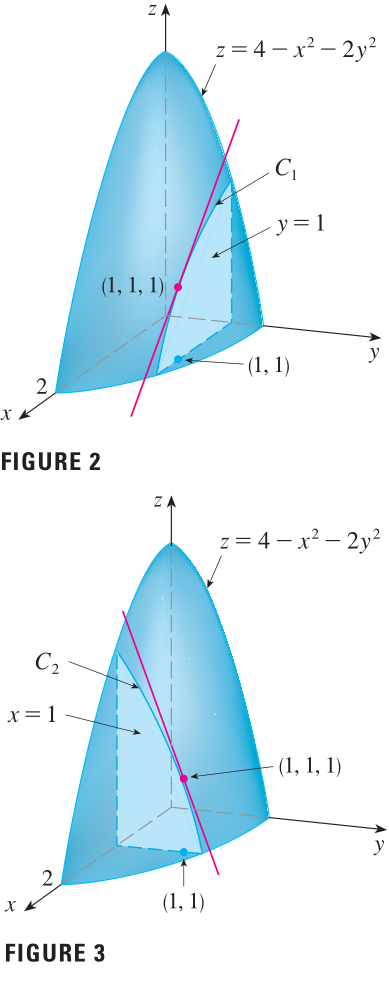
\includegraphics[width = 4  cm]{./images/pareg2.png}
  
\end{minipage}
\begin{minipage}[b]{0.63\linewidth}

 {\fontfamily{lmtt}\selectfont \textbf{\textcolor{blue5}{{\small \faIcon{map-marker-alt}} EXAMPLE.}}} If $f(x,y) = x^3 + x^2 y^3 - 2 y^2 $, find $f_x (1,1)$ and $f_y (1,1)$ and interpret these numbers as slopes.

 We have 
 \begin{equation*}
   \begin{split}
      f_x (x,y) = -2x & \quad \text{ } \quad f_y (x.y) = -4y \\
      f_x(1,1) = -2 & \quad  \text{ } \quad f_y(1,1) = -4  
   \end{split}
 \end{equation*}
 
 The vertical plane $y = 1 $ intersects $f(x,y)$ in the parabola $z = 2 - x^2 $, $y = 1$ ($C_1$). The slope of the tangent line to this parabola at the point $(1,1,1)$ is $f_x (1,1) = -2 $.
\end{minipage}\\
{\fontfamily{lmtt}\selectfont \textbf{\textcolor{blue5}{{\small \faIcon{map-marker-alt}} EXAMPLE.}}} If $f(x,y) = \sin{\left(\cfrac{x }{1 + y }\right)}$, calculate $\cfrac{\delta f }{\partial x }$ and $\cfrac{\delta f}{\partial y}$.

\textcolor{blue5}{\small $ \blacksquare$} Using the Chain Rule for functions of one variable, we have 
\begin{equation*}
  \begin{split}
    & \frac{\partial f }{\partial x } = \cos{\left( \frac{x }{ 1 + y }  \right)} \cdot \frac{\partial}{\partial x } \left( \frac{x }{1 + y }  \right) = \cos{ \left( \frac{x }{1 + y }\right)} \cdot \frac{1 }{1 + y } \\ 
    & \frac{\delta f }{\partial y } = \cos{\left( \frac{x }{ 1 + y }  \right)} \cdot \frac{\partial }{\partial y } \left( \frac{x }{1 + y }  \right) = -  \cos{ \left( \frac{x }{1 + y }\right)} \cdot \frac{x }{(1 + y)^2 } 
  \end{split}
\end{equation*}
{\fontfamily{lmtt}\selectfont \textbf{\textcolor{blue5}{{\small \faIcon{map-marker-alt}} EXAMPLE.}}} Find $\partial z / \partial x $ and $ \partial z / \partial y $ of $z $ is defined as follow 
\[x ^ 3 + y ^ 3 + z ^ 3 + 6 xyz = 1 \]


\begin{minipage}[b]{0.28\linewidth}
  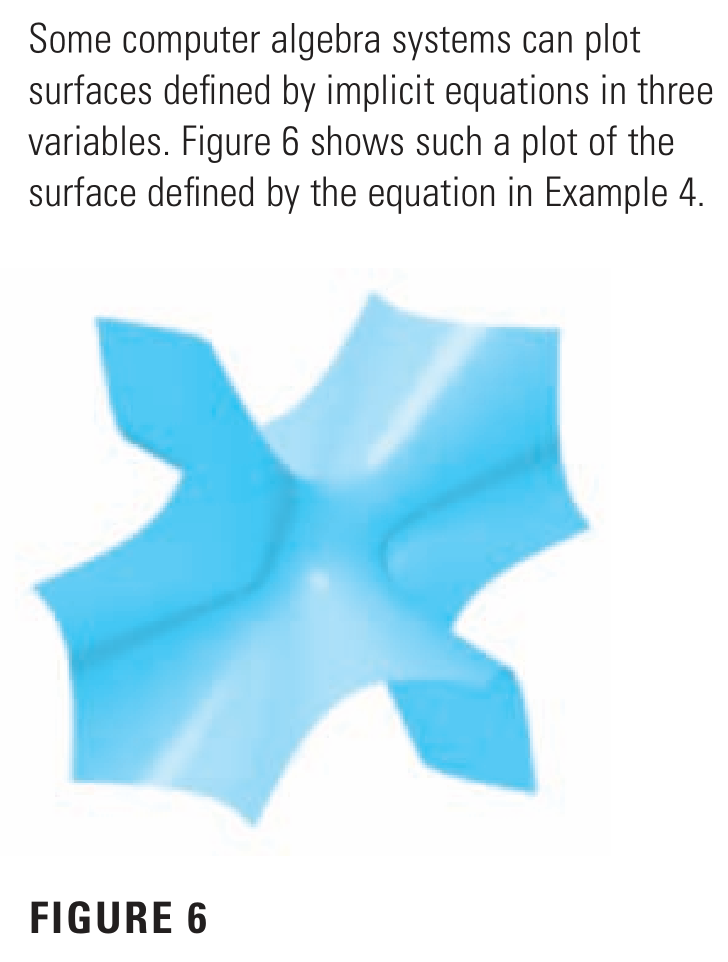
\includegraphics[width = 4.3 cm]{./images/partialeg4.png}
  \end{minipage}
\begin{minipage}[b]{0.67\linewidth}
\textcolor{blue9}{\small $\blacksquare$} First differentiate implicitly with respect to $x $, treat $y $ as a constant.
\[3 x^2 + 3 z^2 \frac{\partial z }{ \partial x } + 6yz + 6xy \frac{\partial z }{ \partial x }= 0\]
Solving this for $\partial z / \partial x $, we obtain 
\[ \frac{\partial z }{\partial x } = - \frac{y^2 + 2xz }{z^2 + 2xy }\]
Similarly, implicit differentiation with respect to $y $ gives 
\[\frac{\partial z }{\partial y } = - \frac{y^2 + 2xz }{z^2 + 2xy }\]
\end{minipage}

\subsection*{{\fontfamily{lmss}\selectfont \underline{Functions of More Than Two Variables }}}  
Regarding $y$ and $z$ as constants and differentiating with respect to $x$.
\[f_x (x, y, z) = \lim_{h \to 0 } \frac{f(x + h, y, z) - f(x,y,z)}{h }\]
{\fontfamily{lmtt}\selectfont \textbf{\textcolor{blue5}{{\small \faIcon{map-marker-alt}} EXAMPLE.}}}  Find $f_x, f _ y $, and $f _ z $ if $f(x,y,z) = e^{xy} \ln{z}$.

Holding $y$ and $z $ constant and differentiating with respect to $x $, we have 
\[f_x = y e^{xy} \ln{z}\]

Similarly, \[f_y = x e^{xy} \ln {z} \quad  \text{and} \quad f_z = \cfrac{e^{xy}}{z }\]

\subsection*{{\fontfamily{lmss}\selectfont \underline{Higher Derivatives}}}

If $f$ is a function of 2 variables, then $f_x$ and $f _ y $ are also functions of 2 variables.  So we can consider the \textbf{second partial derivatives} of $f$, that is $(f_x)_x$, $(f_x)_y $, $(f_y)_x $, and $(f_y)_y $.
\begin{equation*}
  \begin{split}
    & (f _ x ) _ x = f _ {xx} = f _ {11} = \frac{\partial }{\partial x } \left( \frac{\partial f }{ \partial x }\right) = \frac{\partial ^2 f }{\partial  x^2 } = \frac{\partial ^2 z }{\partial x^2 } \\
    & (f _ x ) _ y = f _ {xy} = f _ {12} = \frac{\partial }{\partial y } \left( \frac{\partial f }{ \partial x }\right) = \frac{\partial ^2 f }{\partial  y \text{ } \partial x } = \frac{\partial ^2 z }{\partial y \text{ }\partial x } \\
    & (f _ y ) _ x = f _ {yx} = f _ {21} = \frac{\partial }{\partial x } \left( \frac{\partial f }{ \partial y }\right) = \frac{\partial ^2 f }{\partial  x \text{ } \partial y } = \frac{\partial ^2 z }{\partial x \text{ }\partial y } \\
& (f _ y ) _ y = f _ {yy} = f _ {22} = \frac{\partial }{\partial y } \left( \frac{\partial f }{ \partial y }\right) = \frac{\partial ^2 f }{\partial  y^2 } = \frac{\partial ^2 z }{\partial y^2 }
  \end{split}
\end{equation*}
Thus $f_{xy}$ (or $\partial ^2 f / \partial y \text{ } \partial x $) means that we first differentiate with respect to $x $ and then with respect to $y $.\\
{\fontfamily{lmtt}\selectfont \textbf{\textcolor{blue5}{{\small \faIcon{map-marker-alt}} EXAMPLE.}}} Find the second partial derivatives of 
\[f(x,y) = x ^ 3 + x^2 y^3 - 2 y^2 \]
{\fontfamily{lmss}\selectfont \textcolor{blue5}{\small SOLUTION}} We find that 
\[f_x(x,y) = 3 x^2 + 2x y^3 \quad \text{ } \quad f_y(x,y) = 3 x^2 y^2 - 4y \]
Therefore 
\begin{equation*}
  \begin{split}
    f _ {xx} = \frac{\partial }{\partial x } (3 x^2 + 2xy^3)  = 6x + 2 y^3 & \quad \text{ }  \quad f _ {xy} = \frac{\partial }{ \partial y } (3 x^2 + 2 x y^3) = 6x y^2 \\
    f _ {yx} = \frac{\partial }{\partial x } (3 x^2 y^2 - 4y) = 6x y^2 & \quad \text{ } \quad f_{yy} = \frac{\partial }{\partial y } (3 x^2 y^2 - 4y ) = 6 x^2 y - 4 
  \end{split}
\end{equation*}
\begin{mdframed}
  \textbf{\textcolor{pink}{\fontfamily{lmss}\selectfont Clairaut's Theorem}} $\quad$ Suppose $f $ is defined on a disk $D $ that contains the point $(a, b )$. If the functions $f _ {xy}$ and $f _ {yx }$ are both continuous in $D $, then 
  \[f _ {xy} (a, b) = f _ {yx} (a, b )\]
\end{mdframed}
Partial derivatives of order 3 or higher can also be defined
\[f _ {xyy} = (f _ {xy}) _ y = \frac{\partial }{ \partial y } \left( \frac{\partial ^2 f }{\partial x \text{ } \partial y }\right) = \frac{\partial ^3 f }{\partial y^2 \text{ } \partial x}\]
and using Clairaut's Theorem it can be shown that $f _ {xyy} = f _ {y xy} = f _ {yy x }$. \\
{\fontfamily{lmtt}\selectfont \textbf{\textcolor{blue5}{{\small \faIcon{map-marker-alt}} EXAMPLE.}}} Calculate $f _ {xxyz}$ if $f(x,y,z) = \sin{3x + yz}$. \\
\textbf{\textcolor{blue5}{\fontfamily{lmss}\selectfont \small SOLUTION.}} $\quad $ 
\begin{equation*}
  \begin{split}
     f _ {x} & = 3 \cos{(3x + yz) } \\
     f _ {xx} & = -9 \sin{(3x + yz)} \\
     f _ {xxy} & = -9z \cos{(3x + yz)} \\
     f _ {xxyz} & = -9 \cos{(3x + yz)} + 9yz \sin{(3x + yz)}
  \end{split}
\end{equation*}

\subsection*{{\fontfamily{lmss}\selectfont \underline{Partial Differential Equations}}}
\textbf{Laplace's equation.}
$$\cfrac{\partial ^2 u }{\partial x^2 } + \cfrac{\partial ^2 u }{\partial y^2 } = 0 $$

\section{Tangent Planes and Linear Approximations}
As we zoom in toward a point on a surface of a differentiable function, the surface looks more and more like a plane (its tangent plane) and we can approximate it by a linear function of 2 variables.

\begin{minipage}[b]{0.34\linewidth}
  \begin{center}
    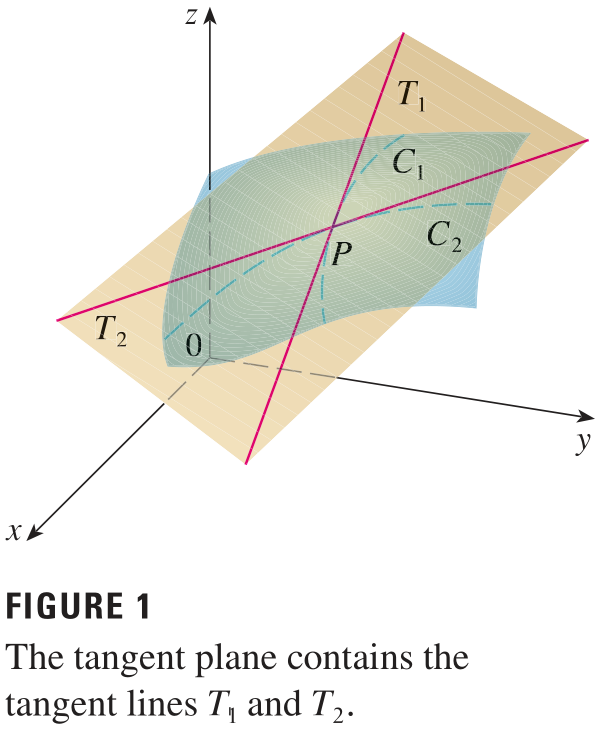
\includegraphics[width = 4.3 cm]{./images/tangentplane.png} 
  \end{center}
  
\end{minipage}
\begin{minipage}[b]{0.63\linewidth}
  \subsection*{{\fontfamily{lmss}\selectfont \underline{Tangent Planes}}}
  Suppose surface $S$ of $z = f(x,y)$ has continuous first partial derivatives, let $P(x _ 0,  y _ 0, z _ 0 ) \in S$. \\
  \textcolor{blue5}{$\blacksquare$} $C _ 1 $ and $C _ 2 $ be the curves obtained by intersecting the vertical planes $y = y _ 0 $ and $ x = x0 $ with $S $.\\
 \textcolor{blue5}{$\blacksquare$} Let $T _ 1 $  and $T _ 2 $ be the tangent lines to the curves  $C _ 1 $ and $ C _ 2$ at $P$. 
 Then the \textbf{tangent plane} to the surface $S $ at the point $P $ contains $T _ 1 $ and $T _ 2 $. In fact, it consists of \textit{all possible} tangent lines at $P $.\\
\textcolor{blue5}{$\blacksquare$} We know the plane has an equation of the form 
\[A(x - x _ 0) + B(y - y _ 0) + C(z - z _ 0 ) = 0 \]
By dividing this by $C $ and letting $a = -A/C $ and $b = -B/C $, 
\[z - z _ 0 =  a(x - x _ 0 ) + b (y - y _ 0 )\]
\end{minipage}

The tangent plane's intersection with the plane $y = y _ 0 $ must be the tangent line $T _ 1 $.
\[z - z _ 0 = a(x - x _ 0 ) \quad \text{ where } y = y _ 0\]

This is a line with slope $a = f _ x (x _ 0, y _ 0  )$. Similarly, $z - z _ 0 = b ( y - y _ 0 )$, and $b = f _ y (x _ 0, y _ 0 )$.

\begin{Def}[Equation of Tangent Plane]
  Suppose $f $ has continuous partial derivatives. An equation of the tangent plane to the surface $z = f(x,y) $ at the point $P(x _ 0, y _ 0, z  _ 0 )$ is 
  \[z - z _ 0 = f_x(x _ 0, y _ 0) (x - x _ 0) + f_y (x _ 0, y _ 0) (y - y _ 0 )\]
\end{Def}
{\fontfamily{lmtt}\selectfont \textbf{\textcolor{blue5}{{\small \faIcon{map-marker-alt}} EXAMPLE.}}} Find the tangent plane to the elliptic paraboloid $z = 2 x^2  + y^2 $ at the point (1, 1, 3).
\begin{align*}
  &f_x(x,y) = 4x & & f_y(x,y) = 2y \\ 
  &f_x(1,1) = 4 & & f_y(1,1) = 2 
\end{align*}    
Then the equation of the tangent plane at (1, 1, 3) is 
\begin{equation*}
  \begin{split}
    z - 3 & = 4(x-1) + 2(y - 1) \\
    z & = 4x + 2y - 3 
  \end{split}
\end{equation*}
\begin{center}
  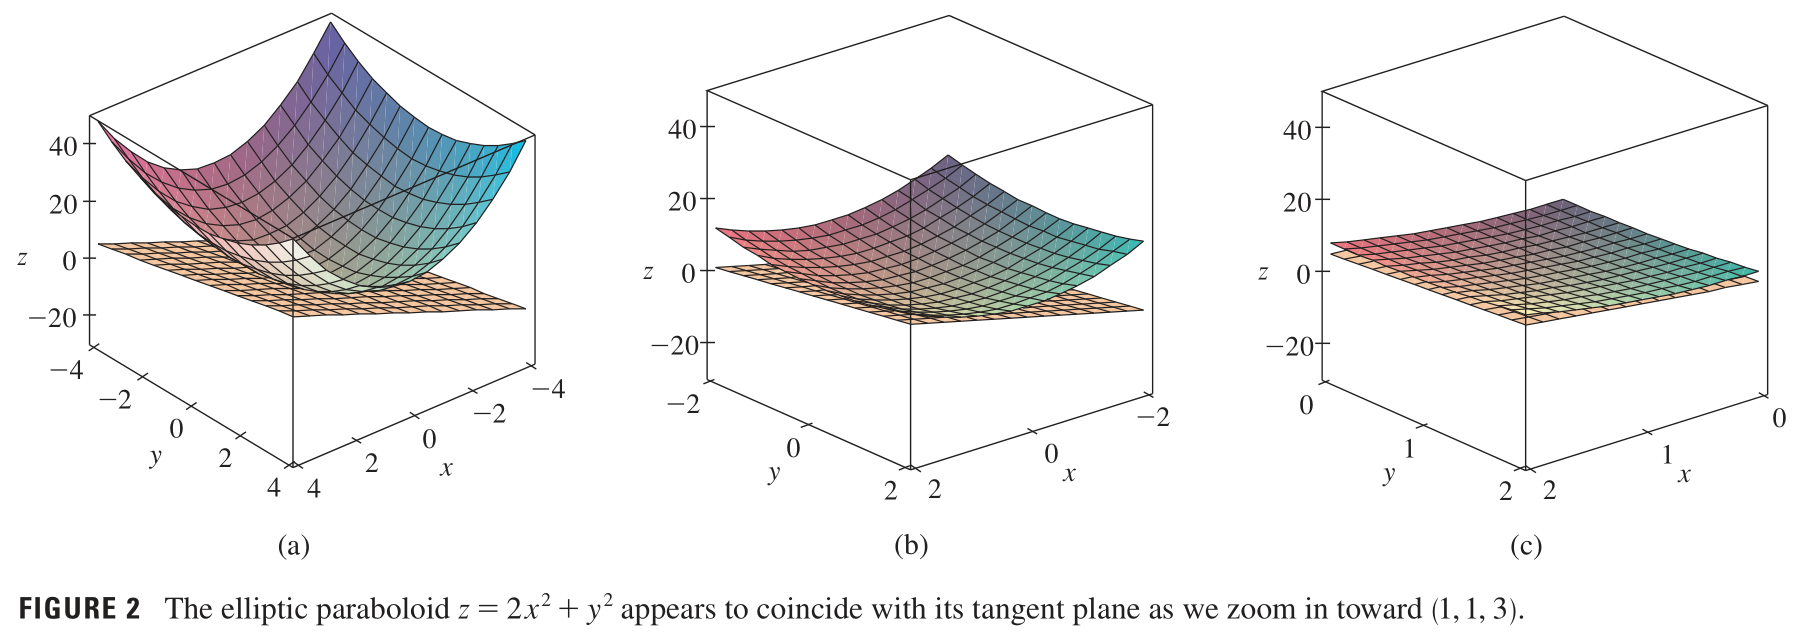
\includegraphics[width = 16 cm]{./images/tangent1.png} 
\end{center}

\begin{minipage}[]{0.34\linewidth}
\hfill  
\end{minipage}
\begin{minipage}[]{0.63\linewidth}
  By zooming toward the point $(1, 1)$ on a contour map, we see that the more we zoom in, the more the level curves look like equally spaced parallel lines.
\end{minipage}

\begin{center}
  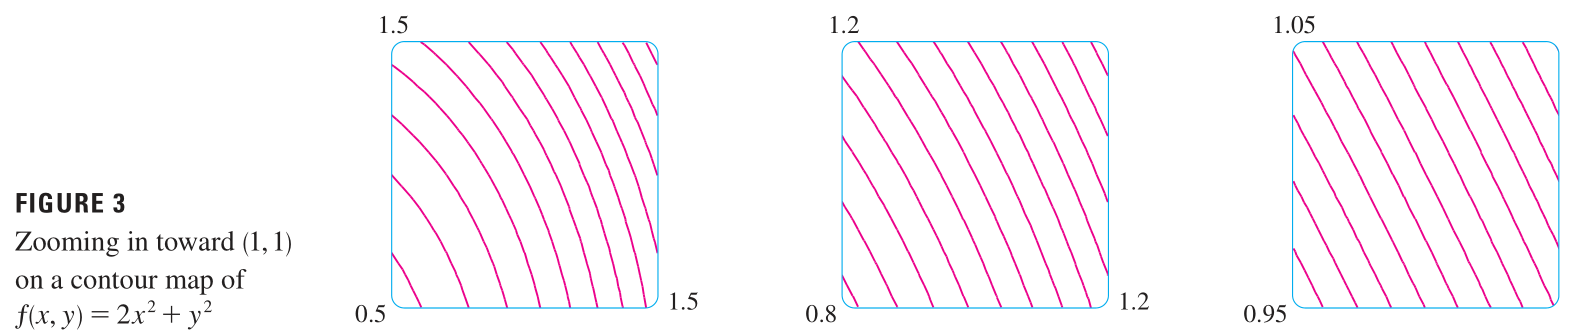
\includegraphics[width = 16 cm]{./images/tangent2.png } 
\end{center}

\begin{minipage}[]{0.54\linewidth}
\subsection*{{\fontfamily{lmss}\selectfont \underline{Linear Approximations}}}
The equation of the tangent plane of $f(x,y) = 2 x^2 + y^2 $ at the point (1, 1, 3) is $z = 4x + 2y - 3 $. Therefore, the linear function of 2 variables 
\[L(x,y) = 4x + 2y - 3 \]
is the \textit{linearization of f} at (1, 1) and the approximation 
\[f(x,y) \approx 4x + 2y - 3 \]
is the \textit{linear approximation} or \textit{tangent plane approximation} of $f$ at (1, 1).
\end{minipage} \hfill
\begin{minipage}[]{0.42\linewidth}
  \begin{mdframed}
Eg: At the point $(1.1,0.95)$, the linear approximation gives 
\[f(1.1,0.95) \approx 4(1.1) + 2(0.95) - 3 = 3.3\]
True value: $f(1.1, 0.95) = 2(1.1)^2 + (0.95)^2 = 3.3225$.
  \end{mdframed}
\end{minipage}

\begin{Def}[]
\textbf{\textcolor{blue5}{\fontfamily{lmss}\selectfont The linearization of $f$ at $(a,b)$.}} $L(x,y) = f(a,b) + f _ x (a,b) (x-a) + f _ y (a,b)(y-b)$\\
\textbf{\textcolor{blue5}{\fontfamily{lmss}\selectfont The linear approximation of $f$ at $(a,b)$.}} $f(x,y) \approx f(a,b) + f _ x (a,b) (x-a) + f _ y (a,b)(y-b)$
\end{Def}

\begin{minipage}[]{0.34\linewidth}
  \begin{center}
    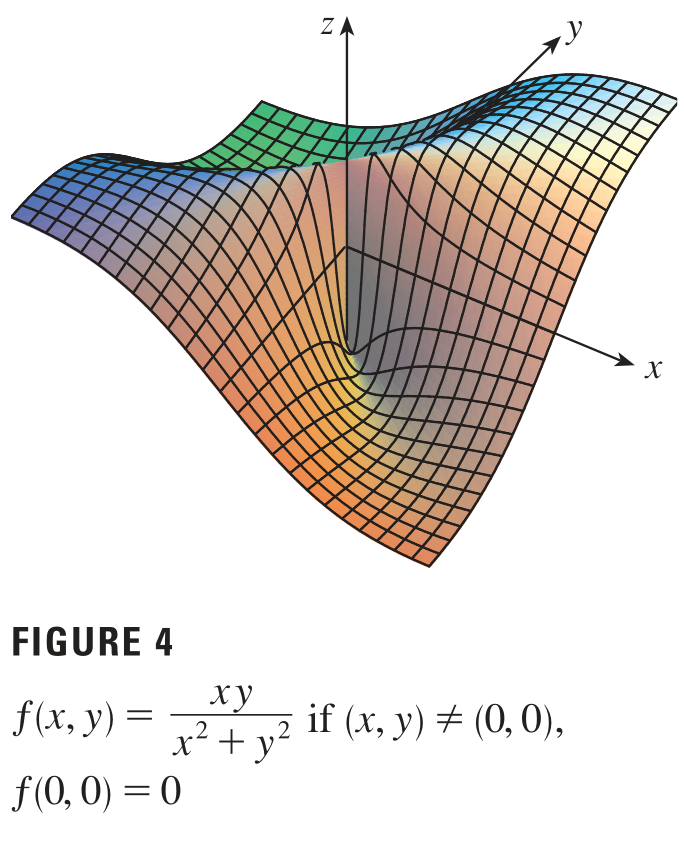
\includegraphics[width = 4.3 cm]{./images/linear.png}
    
  \end{center}
  
\end{minipage}
\begin{minipage}[]{0.63\linewidth}
What if $f _ x $ and $ f _ y $ are not continuous? 
\[f(x,y) = \begin{cases}
  \cfrac{xy }{x^2 + y^2 }& \text{ if } (x,y) \ne (0,0) \\
  0 & \text{ if } (x,y) = (0,0)
\end{cases}\]
Even though $f_x (0,0) = f_y (0,0) = 0$, but they are not continuous.
The linear approximation would be $f(x,y) \approx 0 $, but $f(x,y) = \frac{1 }{2 }$ at all points on the line $y = x $. So we define it as follow.
\end{minipage}

\begin{Def}[Differentiable]
  If $z = f(x,y)$, then $f $ is \textbf{differentiable} at $(a,b)$ if $\Delta z $ can be expressed as 
  \[\Delta z = f_x (a,b) \Delta x + f_y(a,b) \Delta y + \varepsilon _1 \Delta x + \varepsilon _2 \Delta y \]
  where $\varepsilon _ 1 $ and $ \varepsilon _ 2 \to 0$ as $(\Delta x, \Delta y) \to (0,0)$ .
\end{Def}
Pretty ..dumb.
\begin{mdframed}
  \textbf{\textcolor{blue5}{\fontfamily{lmss}\selectfont Theorem.}} If $f_x$ and $f_y $ exist near $(a,b)$ and are continuous at $(a,b)$, then $f $ is differentiable at $(a,b)$.
\end{mdframed}
\begin{minipage}[]{0.28\linewidth}
  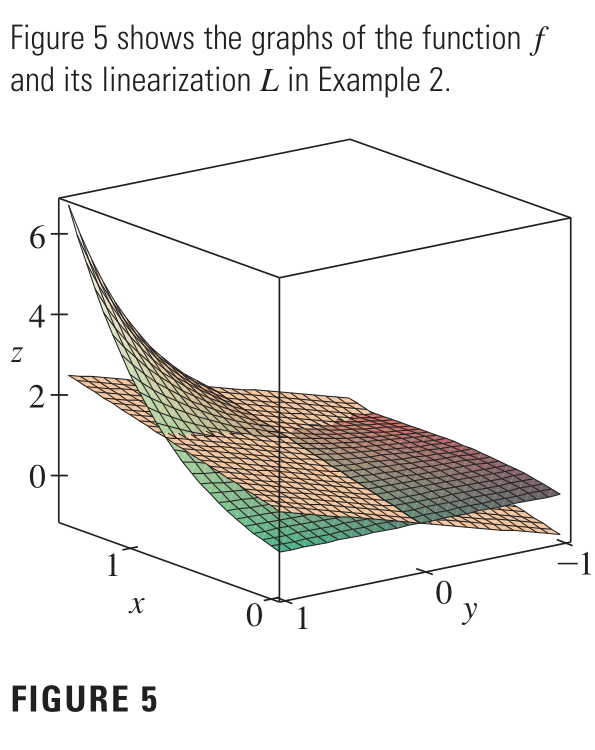
\includegraphics[width = 4.3 cm]{./images/leg2.png}
  
\end{minipage}\hfill
\begin{minipage}[]{0.69\linewidth}
  {\fontfamily{lmtt}\selectfont \textbf{\textcolor{blue5}{{\small \faIcon{map-marker-alt}} EXAMPLE.}}} Show that $f(x,y) = xe^{xy}$ is differentiable at  (1,0) and find its linearization there. Approximate f(1.1, -0.1).

  The partial derivatives are 
  \begin{align*}
    & f_x(x,y) = e^{xy} + x y e^{xy} & & f_x(x,y) = x^2 e^{xy} \\
    & f_x(1,0)  = 1 & & f_y(1,0) = 1
  \end{align*}  
  Both $f_x$ and $f_y $ are continuous, so by the above Theorem, we got $f$ differentiable. The linearization is 
  \begin{align*}
    L(x,y) & = f(1,0) + f_x (1,0)(x-1) + f _ y (1,0)(y - 0) \\
           & = x + y 
  \end{align*}
  So $f(1.1, -0,1) \approx 1.1 - 0.1 = 1 $, actual value: $0.98542 $.
\end{minipage}

\begin{minipage}[]{0.3\linewidth}
  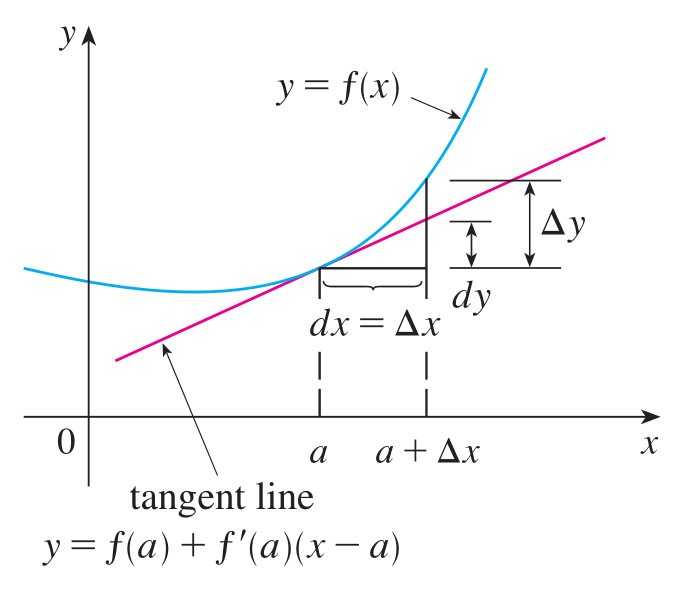
\includegraphics[width = 4.3 cm]{./images/tangentline.png}
\end{minipage}
\begin{minipage}[b]{0.67\linewidth}
\subsection*{{\fontfamily{lmss}\selectfont \underline{\textcolor{blue5}{Differentials}}}}
\textcolor{blue5}{$\blacksquare$} For $y = f(x)$, we define $dx$ an independent variable. And $dy = f'(x)\,dx$, represents the change in height when $x$ changes $dx$. 

\textcolor{blue5}{$\blacksquare$} For a differentiable $z  = f(x,y )$, we define the \textbf{differentials} $dx $ and $dy $ to be independent variables.


\end{minipage}

\begin{Def}[Total differential]
  
Then the \textbf{differential} $dz$ (the \textbf{total differential}), is defined as follow.
  \[dz = f_x(x,y)\,dx + f_y(x,y)\,dy = \cfrac{\partial z }{\partial x }\, dx + \cfrac{\partial z }{ \partial y }\, dy \]
\end{Def}
If we take $dx = \Delta x = x - a $ and $dy = \Delta y = y - b $, then $f(x,y) \approx f(a,b) + dz $.

\begin{center}
  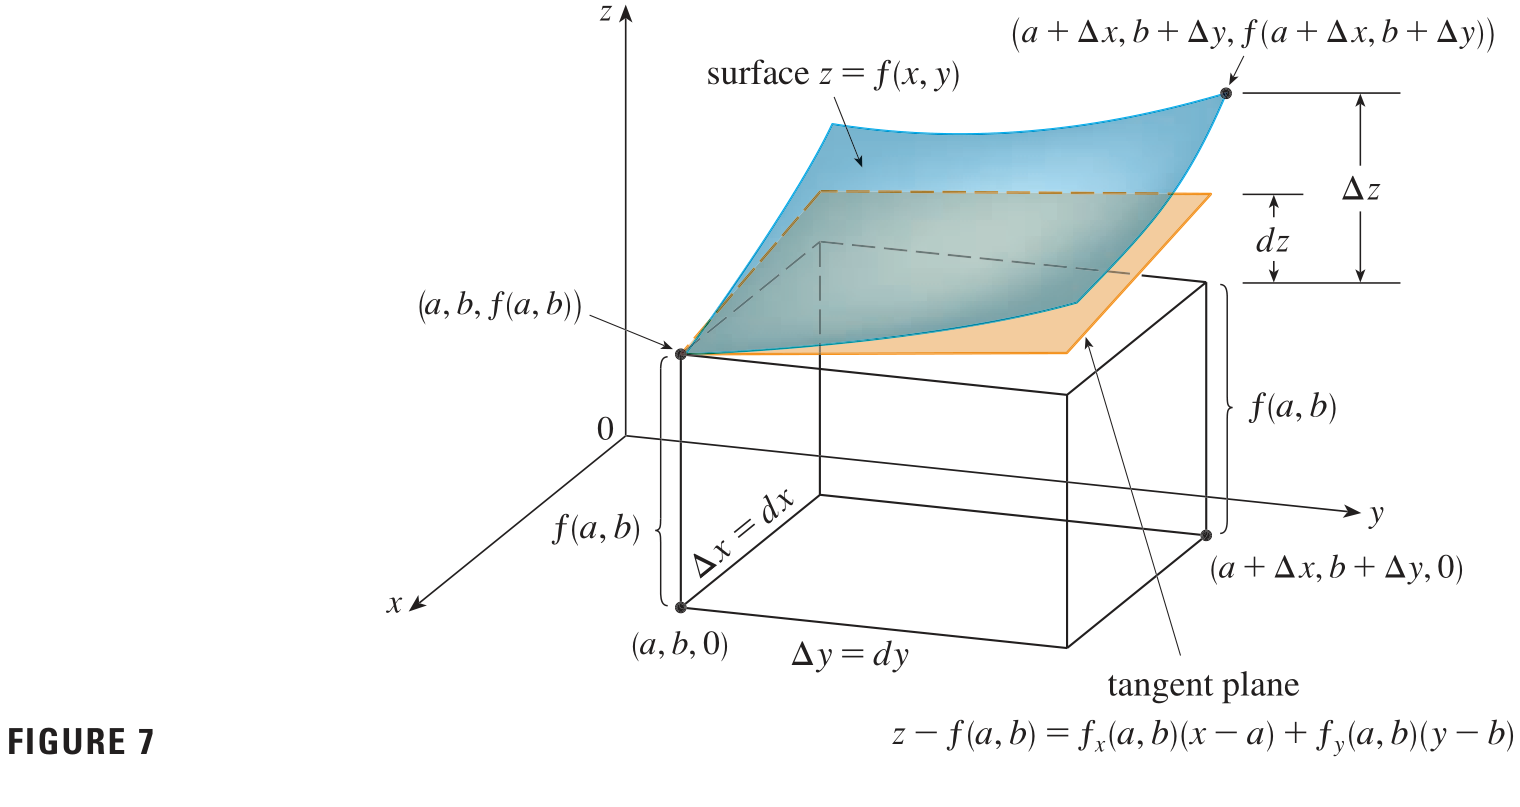
\includegraphics[width = 13 cm]{./images/tangentplaneapp.png} 
\end{center}

\begin{minipage}[]{0.3\linewidth}
  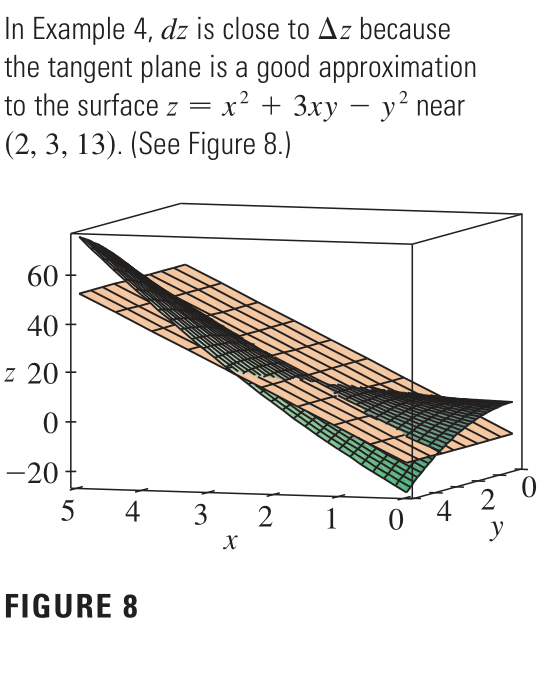
\includegraphics[width = 4.3 cm]{./images/fig8.png}
\end{minipage}
\begin{minipage}[]{0.64\linewidth}
  {\fontfamily{lmtt}\selectfont \textbf{\textcolor{blue5}{{\small \faIcon{map-marker-alt}} EXAMPLE.}}} \\
  (a) If $z = f(x,y) = x^2 + 3xy - y^2 $, find the differential $dz $.\\
  (b) If $x $ changes from 2 to 2.05 and $y $ changes from 3 to 2.96, comppare the values of $\Delta z $ and $dz$.

  \noindent
  {\fontfamily{lmtt}\selectfont \textbf{\textcolor{blue5}{SOLUTION}}} \\
  (a) Applying the formula, \[dz = \,dy = \cfrac{\partial z }{\partial x }\, dx + \cfrac{\partial z }{ \partial y }\, dy = (2x + 3y) \,dx + (3x - 2y)\,dy\]
  (b) Putting $x = 2, \,dx = \Delta x = 0.05, y = 3, dy = \Delta y = -0.04$, we get
  \[dz = [2(2) + 3 (3)]0.05 + [3(2) - 2(3)](-0.04) = 0.65\]
  The increment of $z $ is 
  \begin{align*}
    \Delta z & = f(2.05, 2.96) - f(2,3) \\
             & = [(2.05)^2 + 3(2.05)(2.96) - (2.96)^2] - [2^2 + 3(2)(3) - 3^2] \\
             &= 0.6449
  \end{align*}
{\small \faIcon{greater-than}}
Notice that $\Delta z \approx dz$ but $dz $ is easier to compute.

\end{minipage}

\subsection*{{\fontfamily{lmss}\selectfont \underline{Functions of Three or More Variables}}}
\textbf{Linear approximation.} $f(x,y,z) \approx f(a,b,c) + \Sigma f_x (a,b,c)(x-a)$ \\
\textbf{Total differential.} $dw = \cfrac{\partial w }{\partial x }\, dx + \cfrac{\partial w }{ \partial y }\, dy + \cfrac{\partial w }{\partial z } \,dz$

\section{The Chain Rule}
\begin{Def}[The Chain Rule (Case 1)]
  Suppose that $z = f(x,y)$ is differentiable, where $x = g(t)$ and $y = h(t)$ are both differentiable. Then $z $ is a differentiable function of $t $ and 
  \[\cfrac{dz}{dt } = \cfrac{\partial f }{ \partial x } \, \cfrac{dx }{dt } + 
  \cfrac{\partial f }{\partial y }\, \cfrac{dy }{ dt }\]
\end{Def}

\begin{minipage}[]{0.3\linewidth}
  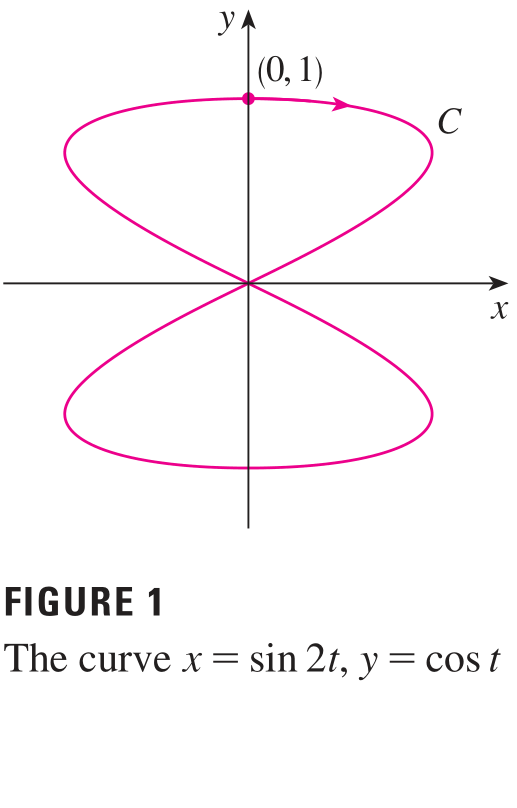
\includegraphics[width = 4.0 cm]{./images/sin2tcost.png}
  
\end{minipage}
\begin{minipage}[]{0.65\linewidth}
{\fontfamily{lmtt}\selectfont \textbf{\textcolor{blue5}{\faIcon{map-marker-alt} EXAMPLE.}}} 
If $z = x^2 y + 3x y^4 $, where $x = \sin{2t}$ and $y = \cos{t}$, find $dz/dt $ when $t = 0 $.

The Chain Rule gives 
\begin{align*}
  \cfrac{dz }{dt } & = \cfrac{\partial f }{ \partial x } \, \cfrac{dx }{dt } + \cfrac{\partial f }{\partial y }\, \cfrac{dy }{ dt } \\
                   & = (2xy + 3y^4)(2\cos{2t}) + (x^2 + 12xy^3)(-\sin{t})
\end{align*}
When $t = 0 $, $x = \sin{0} = 0$ and $y = \cos{0} = 1 $. Therefore 
\[\cfrac{dz }{dt } \Bigg|_{t = 0} = (0 + 3)(2 \cos{0}) + (0 + 0)(-0) = 6 \]
  
\end{minipage}

\begin{Def}[The Chain Rule (Case 2)]
  Suppose that $z = f(x,y)$ is differentiable, where $x = g(s,t)$ and $y = h(s,t)$ are differentiable. We can hold the the other variable fixed.
  \[\cfrac{dz}{ds } = \cfrac{\partial f }{ \partial x } \, \cfrac{dx }{ds } + \cfrac{\partial f }{\partial y }\, \cfrac{dy }{ ds } \quad \text{ } \quad \cfrac{dz}{dt } = \cfrac{\partial f }{ \partial x } \, \cfrac{dx }{dt } + 
  \cfrac{\partial f }{\partial y }\, \cfrac{dy }{ dt }\]
\end{Def}
{\fontfamily{lmtt}\selectfont \textbf{\textcolor{blue5}{\faIcon{map-marker-alt} EXAMPLE.}}} If $z = e^x \sin{y}$, where $x = st^2$, and $y = s^2 t $, find $\partial z/ \partial s $ and $ \partial z / \partial t $.

Applying Case 2 of the Chain Rule, we get 
\begin{align*}
  \cfrac{\partial z }{\partial s } & = \cfrac{\partial f }{ \partial x } \, \cfrac{\partial x }{\partial s } + \cfrac{\partial f }{\partial y }\, \cfrac{\partial y }{ \partial s } = (e^x \sin{y})(t^2) + (e^x \cos{y})(2st) \\
                                   & = t^2 e^{st^2} \sin{(s^2t)} + 2ste^{st^2}\cos{(s^2t)} \\
  \cfrac{\partial z }{\partial t } & = \cfrac{\partial f }{ \partial x } \, \cfrac{\partial x }{\partial t } + \cfrac{\partial f }{\partial y }\, \cfrac{\partial y }{ \partial t } = (e^x \sin{y})(2st) + (e^x \cos{y})(s^2) \\
                                   & = 2ste^{st^2} + s^2 e^{st^2}\cos{s^2t}
\end{align*}

\begin{minipage}[]{0.28\linewidth}
 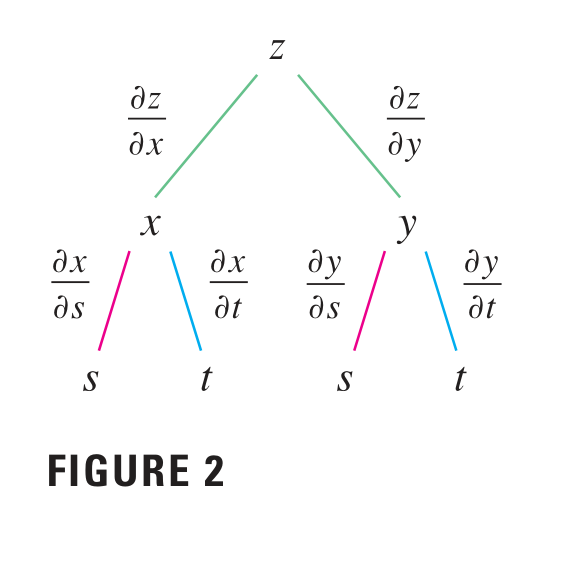
\includegraphics[width = 4 cm]{./images/dxyzt.png}
  
\end{minipage}
\begin{minipage}[]{0.69\linewidth}
\textcolor{purple}{\faIcon{greater-than} \textbf{{\fontfamily{lmtt}\selectfont Note.}}}
 $s, t $ are \textbf{independent} variables, $x, y $ are \textbf{intermediate} variables, and $z $ is the \textbf{dependent} variable.

 For the gemeral version of $n$ variables, it's similar.

  
\end{minipage}\\
{\fontfamily{lmtt}\selectfont \textbf{\textcolor{blue5}{\faIcon{map-marker-alt} EXAMPLE.}}} If $g(s,t) = f(s^2 - t^2, t^2 - s^2 )$ and $f $ is differentiable, show that $g $ satisfies the equation  \[t \,\cfrac{\partial g }{ \partial s } + s \, \cfrac{\partial g }{ \partial t } = 0\]
{\fontfamily{lmtt}\selectfont \textbf{\textcolor{blue5}{\faIcon{map-marker-alt} EXAMPLE.}}} If $z = f(x,y)$ has continuous second-order partial derivatives and $x = r^2 + s^2 $ and $ y = 2 rs $, find \\
\textbf{a.} $\partial z / \partial r$ \\
\textbf{b.} $\partial ^2 z / \partial r^2 $ \\
{\fontfamily{lmtt}\selectfont \textbf{\textcolor{blue5}{SOLUTION.}}} \\
\textbf{a.} The Chain Rule gives 
\[ \cfrac{\partial z }{\partial r }  = \cfrac{\partial f }{ \partial x } \, \cfrac{\partial x }{\partial r } + \cfrac{\partial f }{\partial y }\, \cfrac{\partial y }{ \partial r } = \cfrac{\partial z }{ \partial x } (2r) + \cfrac{\partial  z }{ \partial y } (2s )\]

\textbf{b.} Applying the Product Rule, we get 
\begin{align*}
  \cfrac{\partial ^2 z }{\partial r^2 } & = \cfrac{\partial }{\partial r } \left( 2r \cfrac{\partial z }{\partial x } + 2s \cfrac{\partial z }{\partial y } \right) \\
  & = 2 \cfrac{\partial z }{\partial x } + 2r \cfrac{\partial }{\partial r } \left( \cfrac{\partial z }{\partial x } \right) + 2s \cfrac{\partial }{\partial r } \left( \cfrac{\partial z }{\partial y } \right)
\end{align*}

\begin{minipage}[]{0.26\linewidth}
  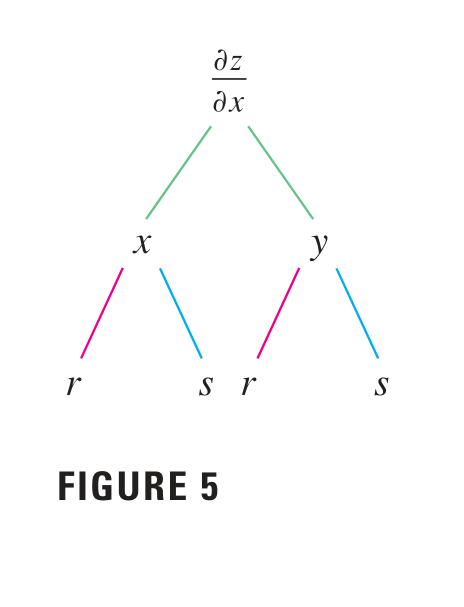
\includegraphics[width = 4 cm]{./images/chainrulefig5.png}
  
\end{minipage}
\begin{minipage}[]{0.69\linewidth}

Using the Chain Rule again (Figure 5), we have 
\begin{align*}
  \cfrac{\partial  }{\partial r  } \left( \cfrac{\partial z }{ \partial x } \right) = \cfrac{\partial }{ \partial x } \left( \cfrac{\partial z }{ \partial x } \right) \cfrac{\partial x }{ \partial r } + \cfrac{\partial }{ \partial y } \left( \cfrac{\partial z }{ \partial x } \right) \cfrac{\partial y }{\partial r }= \cfrac{\partial ^2 z }{\partial x^2 } (2r) + \cfrac{\partial ^2 z }{\partial y \partial x } (2s) \\
  \cfrac{\partial }{ \partial r } \left( \cfrac{\partial z }{ \partial y } \right) = \cfrac{\partial ^2 z }{\partial x \partial y } (2r) + \cfrac{\partial ^2 z }{ \partial y^2 }(2s) 
\end{align*} 
\end{minipage}\\
Putting these into the previous equation, 
\[\cfrac{\partial ^2 z }{\partial r^2 } = 2 \cfrac{\partial z }{\partial x } + 4 r^2 \cfrac{dd^2 z }{\partial x^2 } + 8rs \cfrac{\partial ^2 z }{\partial x \partial y } + 4s^2 \cfrac{\partial ^2 z }{\partial y^2 }\]

\subsection*{{\fontfamily{lmss}\selectfont \underline{Implicit Differentiation}}}
Suppose $F(x,y) = 0 $, $y = f(x)$ is differentiable. If $F $ is differentiable, apply Case 1 of the Chain Rule to differentiate both sides with respect to $x $.
\[\cfrac{\partial F }{\partial x } \cfrac{dx }{ dx } + \cfrac{\partial F }{ \partial y } \cfrac{dy }{dx } = 0\]
\begin{center}
  \begin{minipage}[]{0.3\linewidth}
    \begin{mdframed}
      \[\cfrac{dy }{dx } = - \cfrac{\cfrac{\partial F }{\partial x }}{\cfrac{\partial F }{ \partial y }} = - \cfrac{F_x }{F_y}\]
    \end{mdframed}
  \end{minipage}
\end{center}
{\fontfamily{lmtt}\selectfont \textbf{\textcolor{blue5}{\faIcon{map-marker-alt} EXAMPLE.}}} Find $y' $ if $x^3 + y^3 = 6xy $.

{\fontfamily{lmtt}\selectfont \textbf{\textcolor{blue5}{SOLUTION.}}} $F(x,y) = x^3 + y^3 - 6xy = 0 $ which gives 
\[\cfrac{dy }{dx } = -\cfrac{F_x }{F_y } = - \cfrac{3x^2 - 6y }{3y^2 - 6x } = - \cfrac{x^2 - 2y }{y^2 - 2x }\]

\begin{Def}[Implicit Function Theorem]
  \[\cfrac{\partial z }{\partial x } = - \cfrac{\cfrac{\partial F }{ \partial x }}{\cfrac{\partial F }{\partial z }} \quad \text{ } \quad \cfrac{\partial z }{\partial y } = - \cfrac{\cfrac{\partial F }{\partial y }}{\cfrac{\partial F }{\partial z }}\]
\end{Def}
{\fontfamily{lmtt}\selectfont \textbf{\textcolor{blue5}{\faIcon{map-marker-alt} EXAMPLE.}}} Find $\cfrac{\partial z }{ \partial x }$ and $ \cfrac{\partial z }{\partial y }$ if $x^3 + y ^3 + z^3 + 6xyz = 1 $.

{\fontfamily{lmtt}\selectfont \textbf{\textcolor{blue5}{SOLUTION.}}} 
Let $f(x,y,z) = x^3 + y^3 + z^3 + 6xyz - 1 $, then we have 
\begin{align*}
  \cfrac{\partial z }{ \partial x } = - \cfrac{F_x }{F_z } = - \cfrac{x^2 + 2yz }{z^2 + 2xy } \\
  \cfrac{\partial z }{ \partial y } = - \cfrac{F_y }{F_z } = - \cfrac{y^2 + 2xz }{z^2 + 2xy }
\end{align*}


\end{document}
